 
%----------------------------------------------------------------------------------------
%	PACKAGES AND OTHER DOCUMENT CONFIGURATIONS
%----------------------------------------------------------------------------------------

\documentclass[
12pt, % The default document font size, options: 10pt, 11pt, 12pt
%oneside, % Two side (alternating margins) for binding by default, uncomment to switch to one side
french, % ngerman for German
singlespacing, % Single line spacing, alternatives: onehalfspacing or doublespacing
%draft, % Uncomment to enable draft mode (no pictures, no links, overfull hboxes indicated)
%nolistspacing, % If the document is onehalfspacing or doublespacing, uncomment this to set spacing in lists to single
%liststotoc, % Uncomment to add the list of figures/tables/etc to the table of contents
%toctotoc, % Uncomment to add the main table of contents to the table of contents
%parskip, % Uncomment to add space between paragraphs
%nohyperref, % Uncomment to not load the hyperref package
headsepline, % Uncomment to get a line under the header
%chapterinoneline, % Uncomment to place the chapter title next to the number on one line
%consistentlayout, % Uncomment to change the layout of the declaration, abstract and acknowledgements pages to match the default layout
]{MastersDoctoralThesis} % The class file specifying the document structure
 
 \usepackage{hyperref}
 \hypersetup{
 	colorlinks=true,
 	linkcolor=black,
 	filecolor=black,
 	urlcolor=black,
 	citecolor=black
 }

 
 \AtBeginDocument{\renewcommand{\labelitemi}{%
 		\hspace{3mm}\textbullet}}%pour les numératation avec les puces pour les itemize
\usepackage[utf8]{inputenc} % Required for inputting international characters
\usepackage[T1]{fontenc} % Output font encoding for international characters

\usepackage{mathpazo} % Use the Palatino font by default

\usepackage[backend=bibtex,style=authoryear,natbib=true]{biblatex} % Use the bibtex backend with the authoryear citation style (which resembles APA)

\addbibresource{mybiblio.bib} % The filename of the bibliography

\usepackage[autostyle=true]{csquotes} % Required to generate language-dependent quotes in the bibliography
\usepackage{tcolorbox}
 
%----------------------------------------------------------------------------------------
%	MARGIN SETTINGS
%----------------------------------------------------------------------------------------

\geometry{
	paper=a4paper, % Change to letterpaper for US letter
	inner=2.5cm, % Inner margin
	outer=2.5cm, % Outer margin
	bindingoffset=.5cm, % Binding offset
	top=1.5cm, % Top margin
	bottom=1.5cm, % Bottom margin
	%showframe, % Uncomment to show how the type block is set on the page
}

%----------------------------------------------------------------------------------------
%	THESIS INFORMATION
%----------------------------------------------------------------------------------------

\thesistitle{Thesis Title} % Your thesis title, this is used in the title and abstract, print it elsewhere with \ttitle
\supervisor{Dr. James \textsc{Smith}} % Your supervisor's name, this is used in the title page, print it elsewhere with \supname
\examiner{} % Your examiner's name, this is not currently used anywhere in the template, print it elsewhere with \examname
\degree{Doctor of Philosophy} % Your degree name, this is used in the title page and abstract, print it elsewhere with \degreename
\author{John \textsc{Smith}} % Your name, this is used in the title page and abstract, print it elsewhere with \authorname
\addresses{} % Your address, this is not currently used anywhere in the template, print it elsewhere with \addressname

\subject{Biological Sciences} % Your subject area, this is not currently used anywhere in the template, print it elsewhere with \subjectname
\keywords{} % Keywords for your thesis, this is not currently used anywhere in the template, print it elsewhere with \keywordnames
\university{\href{http://www.university.com}{University Name}} % Your university's name and URL, this is used in the title page and abstract, print it elsewhere with \univname
\department{\href{http://department.university.com}{Department or School Name}} % Your department's name and URL, this is used in the title page and abstract, print it elsewhere with \deptname
\group{\href{http://researchgroup.university.com}{Research Group Name}} % Your research group's name and URL, this is used in the title page, print it elsewhere with \groupname
\faculty{\href{http://faculty.university.com}{Faculty Name}} % Your faculty's name and URL, this is used in the title page and abstract, print it elsewhere with \facname

\AtBeginDocument{
\hypersetup{pdftitle=\ttitle} % Set the PDF's title to your title
\hypersetup{pdfauthor=\authorname} % Set the PDF's author to your name
\hypersetup{pdfkeywords=\keywordnames} % Set the PDF's keywords to your keywords
}

\begin{document}

\frontmatter % Use roman page numbering style (i, ii, iii, iv...) for the pre-content pages

\pagestyle{plain} % Default to the plain heading style until the thesis style is called for the body content

%----------------------------------------------------------------------------------------
%	TITLE PAGE
%----------------------------------------------------------------------------------------

%\begin{titlepage}
%\begin{center}

%\vspace*{.06\textheight}
%{\scshape\LARGE \univname\par}\vspace{1.5cm} % University name
%\textsc{\Large Doctoral Thesis}\\[0.5cm] % Thesis type

%\HRule \\[0.4cm] % Horizontal line
%{\huge \bfseries \ttitle\par}\vspace{0.4cm} % Thesis title
%\HRule \\[1.5cm] % Horizontal line
 
%\begin{minipage}[t]{0.4\textwidth}
%\begin{flushleft} \large
%\emph{Author:}\\
%\href{http://www.johnsmith.com}{\authorname} % Author name - remove the \href bracket to remove the link
%\end{flushleft}
%\end{minipage}
%\begin{minipage}[t]{0.4\textwidth}
%\begin{flushright} \large
%\emph{Supervisor:} \\
%\href{http://www.jamessmith.com}{\supname} % Supervisor name - remove the \href bracket to remove the link  
%\end{flushright}
%\end{minipage}\\[3cm]
 
%\vfill

%\large \textit{A thesis submitted in fulfillment of the requirements\\ for the degree of \degreename}\\[0.3cm] % University requirement text
%\textit{in the}\\[0.4cm]
%\groupname\\\deptname\\[2cm] % Research group name and department name
 
%\vfill

%{\large \today}\\[4cm] % Date
%\includegraphics{Logo} % University/department logo - uncomment to place it
 
%\vfill
%\end{center}
%\end{titlepage}

%----------------------------------------------------------------------------------------
%	DECLARATION PAGE
%----------------------------------------------------------------------------------------

%\begin{declaration}
%\addchaptertocentry{\authorshipname} % Add the declaration to the table of contents
%\noindent I, \authorname, declare that this thesis titled, \enquote{\ttitle} and the work presented in it are my own. I confirm that:

%\begin{itemize} 
%\item This work was done wholly or mainly while in candidature for a research degree at this University.
%\item Where any part of this thesis has previously been submitted for a degree or any other qualification at this University or any other institution, this has been clearly stated.
%\item Where I have consulted the published work of others, this is always clearly attributed.
%\item Where I have quoted from the work of others, the source is always given. With the exception of such quotations, this thesis is entirely my own work.
%\item I have acknowledged all main sources of help.
%\item Where the thesis is based on work done by myself jointly with others, I have made clear exactly what was done by others and what I have contributed myself.\\
%\end{itemize}
 
%\noindent Signed:\\
%\rule[0.5em]{25em}{0.5pt} % This prints a line for the signature
 
%\noindent Date:\\
%\rule[0.5em]{25em}{0.5pt} % This prints a line to write the date
%\end{declaration}

%\cleardoublepage

%----------------------------------------------------------------------------------------
%	QUOTATION PAGE
%----------------------------------------------------------------------------------------

%\vspace*{0.2\textheight}

%\noindent\enquote{\itshape Thanks to my solid academic training, today I can write hundreds of words on virtually any topic without possessing a shred of information, which is how I got a good job in journalism.}\bigbreak

%\hfill Dave Barry

%----------------------------------------------------------------------------------------
%	ABSTRACT PAGE
%----------------------------------------------------------------------------------------

%\begin{abstract}
%\addchaptertocentry{\abstractname} % Add the abstract to the table of contents
%The Thesis Abstract is written here (and usually kept to just this page). The page is kept centered vertically so can expand into the blank space above the title too\ldots
%\end{abstract}

%----------------------------------------------------------------------------------------
%	ACKNOWLEDGEMENTS
%----------------------------------------------------------------------------------------

%\begin{acknowledgements}
%\addchaptertocentry{\acknowledgementname} % Add the acknowledgements to the table of contents
%The acknowledgments and the people to thank go here, don't forget to include your project advisor\ldots
%\end{acknowledgements}

%----------------------------------------------------------------------------------------
%	LIST OF CONTENTS/FIGURES/TABLES PAGES
%----------------------------------------------------------------------------------------

\tableofcontents % Prints the main table of contents

\listoffigures % Prints the list of figures

\listoftables % Prints the list of tables

%----------------------------------------------------------------------------------------
%	ABBREVIATIONS
%----------------------------------------------------------------------------------------

%\begin{abbreviations}{ll} % Include a list of abbreviations (a table of two columns)

%\textbf{LAH} & \textbf{L}ist \textbf{A}bbreviations \textbf{H}ere\\
%\textbf{WSF} & \textbf{W}hat (it) \textbf{S}tands \textbf{F}or\\

%\end{abbreviations}

\chapter*{Liste des abréviations}

%----------------------------------------------------------------------------------------
%	PHYSICAL CONSTANTS/OTHER DEFINITIONS
%----------------------------------------------------------------------------------------

%\begin{constants}{lr@{${}={}$}l} % The list of physical constants is a three column table

% The \SI{}{} command is provided by the siunitx package, see its documentation for instructions on how to use it

%Speed of Light & $c_{0}$ & \SI{2.99792458e8}{\meter\per\second} (exact)\\
%Constant Name & $Symbol$ & $Constant Value$ with units\\

%\end{constants}

%----------------------------------------------------------------------------------------
%	SYMBOLS
%----------------------------------------------------------------------------------------

%\begin{symbols}{lll} % Include a list of Symbols (a three column table)

%$a$ & distance & \si{\meter} \\
%$P$ & power & \si{\watt} (\si{\joule\per\second}) \\
%Symbol & Name & Unit \\

%\addlinespace % Gap to separate the Roman symbols from the Greek

%$\omega$ & angular frequency & \si{\radian} \\

%\end{symbols}

%----------------------------------------------------------------------------------------
%	DEDICATION
%----------------------------------------------------------------------------------------

%\dedicatory{For/Dedicated to/To my\ldots} 

%----------------------------------------------------------------------------------------
%	THESIS CONTENT - CHAPTERS
%----------------------------------------------------------------------------------------

\mainmatter % Begin numeric (1,2,3...) page numbering

%----------------------------------------------------------------------------------------
%	Introduction Général
%----------------------------------------------------------------------------------------
\chapter*{Introduction générale}
\addcontentsline{toc}{chapter}{Introduction générale}




%\pagestyle{headings}
\pagestyle{thesis} % Return the page headers back to the "thesis" style

% Include the chapters of the thesis as separate files from the Chapters folder
% Uncomment the lines as you write the chapters


% Chapter 1

\chapter{Etat de l'art} % Main chapter title

\label{Chapter1} % For referencing the chapter elsewhere, use \ref{Chapter1} 

%----------------------------------------------------------------------------------------

% Define some commands to keep the formatting separated from the content 
\newcommand{\keyword}[1]{\textbf{#1}}
\newcommand{\tabhead}[1]{\textbf{#1}}
\newcommand{\code}[1]{\texttt{#1}}
\newcommand{\file}[1]{\texttt{\bfseries#1}}
\newcommand{\option}[1]{\texttt{\itshape#1}}

%----------------------------------------------------------------------------------------

%----------------------------------------------------------------------------------------
%	Introduction
%----------------------------------------------------------------------------------------

\section{Introduction}



%----------------------------------------------------------------------------------------
%Notion de caméras	
%----------------------------------------------------------------------------------------

\newpage
\section{Notion de caméras}

Une caméra est un dispositif qui capture la lumière et la transforme en image. Elle le fait à travers une lentille, qui concentre la lumière sur une surface sensible à celle-çi, où une image se forme \cite{noauthor_quest-ce_nodate}. \\

 Il ya deux catégories de caméras :
 \begin{itemize}
 	\item \textbf{Les caméras numériques}: qui capturent des images par voie électronique à l’aide d’un capteur.
 	\item\textbf{les caméras à pellicule}: Elles utilisent une bande de pellicule enduit de produits chimiques photosensibles. Elles sont utilisées pour la réalisation de film.
 	La pellicule est une feuille mince formant le support souple à une couche sensible , elle définit chaque détaille d'une photo(couleurs, contrastes, exposition, grain, etc)\\
 \end{itemize}
 
\begin{figure}[h]
	\centering
	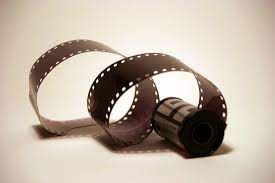
\includegraphics[scale=0.80]{image/pellicule.jpeg}
	\decoRule
	\caption[Pellicule]{image d'une pellicule.}
	\label{fig:Pellicule}
\end{figure}

\subsection{Les parties essentielles d'une caméra}
Les parties essentielles d’une caméra comprennent : \\
\begin{itemize}
	\item \textbf{Le corps :} qui tient l'ensemble de toutes les composantes . \\
	
	\item \textbf{La lentille :} qui met la lumière au centre du capteur d’image. \\
	
	\item \textbf{L’obturateur :} qui contrôle la quantité de lumière qui atteint le capteur.\\ 
	
	\item \textbf{L’ouverture :} qui contrôle la quantité de lumière que l’objectif laisse entrer. \\
	
	\item \textbf{Le capteur d'image:} IL convertit le rayonnement électromagnétique en un signal électrique analogique. Ce signal est ensuite amplifié, puis numérisé par un convertisseur analogique-numérique et enfin traité pour obtenir une image numérique. La taille du capteur de caméra a un impact significatif sur la qualité de l’image.En effet des capteurs plus grands permettent d'avoir généralement une meilleure qualité d’image, surtout dans des conditions d’éclairage faible. Ils ont également une plus grande surface pour la prise de détails, ce qui peut se traduire par des photos plus nettes et plus détaillées.\\
\end{itemize}

\subsection{Le micrologiciel d'une caméra}
Le micrologiciel ou firmware d'une caméra est un type de logiciel programmé dans le matériel de la caméra, il contrôle toutes les fonctions de la caméra,de la mise au point automatique et des paramètres d’exposition jusqu’au traitement et au stockage des images.\\

\subsection{Les différents types de caméras}

ils existes sept types de caméras qui sont entre autre: \cite{noauthor_les_2015} :

\begin{itemize}
	\item \textbf{Les caméras de smartphones} : Ce sont les caméras intégrés dans les téléphones portables.De nos jours la qualité des images qu'elles produisent les amènes à rivaliser avec les caméras professionnels qui existe sur le marché.Elles sont utilisés pour les web vidéos, clips, interviews, courts-métrages, etc......\\
	
	\item \textbf{Les Camescopes} sont des caméras utilisé par le grand public pour leurs souvenirs de famille.Aujord'hui elles sont rare sur le marché car elles sont remplacées par les smartphones.seuls les plus chers parviennent à se démarquer par leur qualité d’image . Elles sont souvent de petite taille, élaborées pour automatiser la plupart des réglages et disposent bien souvent de petits capteurs mais jamais d’entrées audio.\\
		\textbf{Exemple :\\}
    	\begin{itemize}
    		\item Canon Vixia HF R52
    		\item Sony HDR PJ275
    		\item Panasonic HC W850
    	\end{itemize}
    	 
		\begin{figure}[h]
			\centering
		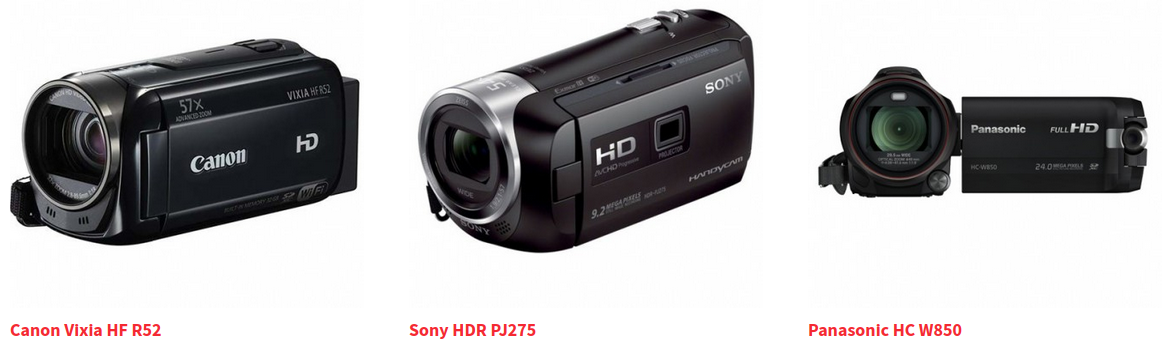
\includegraphics[scale=0.35]{image/camescopes.png}
			\decoRule
			\caption[Camescopes]{image de Camescopes.}
			\label{fig:Camescopes}
		\end{figure}
\newpage
	\item \textbf{Les DSLR(digital single-lens reflex)} sont des appareils photo réflex numériques disposant d’une fonction de capture vidéo.Ils sont caractérisés par la taille de leur capteur qui permettent d'avoir des images de qualités, d’objectifs interchangeables qui permettent de varier les rendus stylistiques en jouant avec les différents types de « cailloux » selon les photographes et la petite taille des lentilles (comparé à ceux d’une caméra pro) rend accessible le prix des objectifs.\\
		\textbf{Exemple :\\}
		\begin{itemize}
			\item Canon 5D Mark III
			\item Nikon D800
			\item Canon 7D
		\end{itemize}
		\begin{figure}[h]
			\centering
			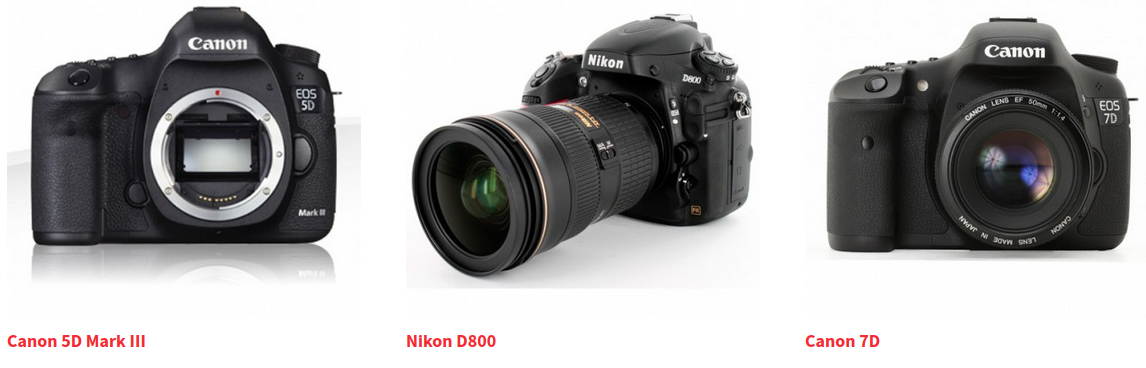
\includegraphics[scale=0.35]{image/DSLR.png}
			\decoRule
			\caption[digital single-lens reflex(DSLR)]{image de digital single-lens reflex(DSLR).}
			\label{fig:digital single-lens reflex(DSLR)}
		\end{figure}
		
		
	\item \textbf{Les Caméras dites « Prosommateurs »} Le mot « prosommateur » est composé de « pro » issu de production et « sommateur » de consommateur. On appelle les prosommateurs les personnes qui achètent des produits avec une certaine exigence car ils ont pour intention d’utiliser le produit dans un cadre de production.Ces caméras assez récentes sont venues perturber la frontière entre camescopes et caméras professionnelles en insérerant une gamme intermédiaire répondant aux besoins des petits producteurs indépendants.Elles sont généralement d’une taille supérieure à un camescope mais bien moins encombrante que les caméras pro de plateau ou de cinéma et proposent une excellente qualité d’image.\\
			\textbf{Exemple :\\}
		\begin{itemize}
			\item Sony PMW 300
			\item Panasonic AG HPX250
			\item Canon XF 205
		\end{itemize}
		\vspace{4 cm}
		\begin{figure}[h]
			\centering
			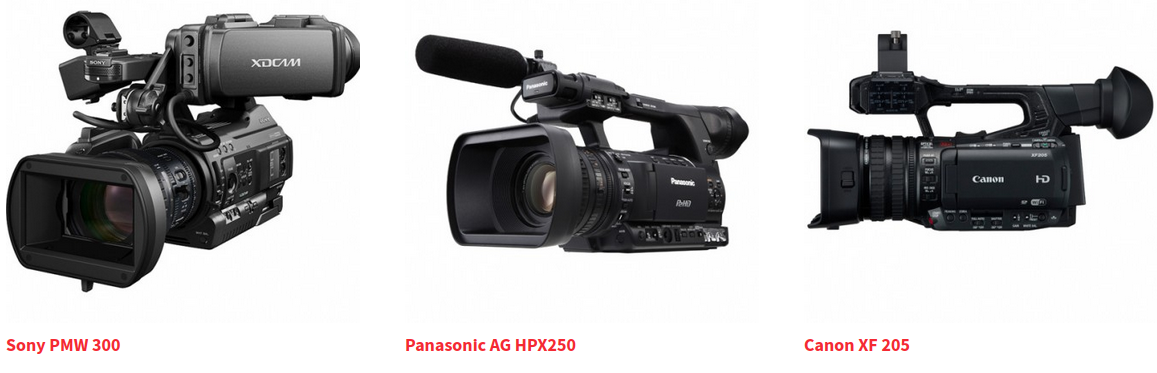
\includegraphics[scale=0.3]{image/prosommateur.png}
			\decoRule
			\caption[Les Caméras dites « Prosommateurs »]{Les Caméras dites « Prosommateurs ».}
			\label{fig:Les Caméras dites « Prosommateurs »}
		\end{figure}
		
	\item \textbf{Caméras Professionnelles} Les caméras professionnelles sont de très grosses caméras disposant des capteurs les plus gros, les objectifs y sont évidemment interchangeables,le paramétrage de la colorimétrie y est bien souvent plus poussé, et elle sont systématiquement synchronisable par timecode. \\
			\textbf{Exemple :\\}
		\begin{itemize}
			\item Panavision Panaflex Millenium
			\item Arri Arriflex D-21
			\item Aaton Penelope
		\end{itemize}
 		
		\begin{figure}[h]
			\centering
			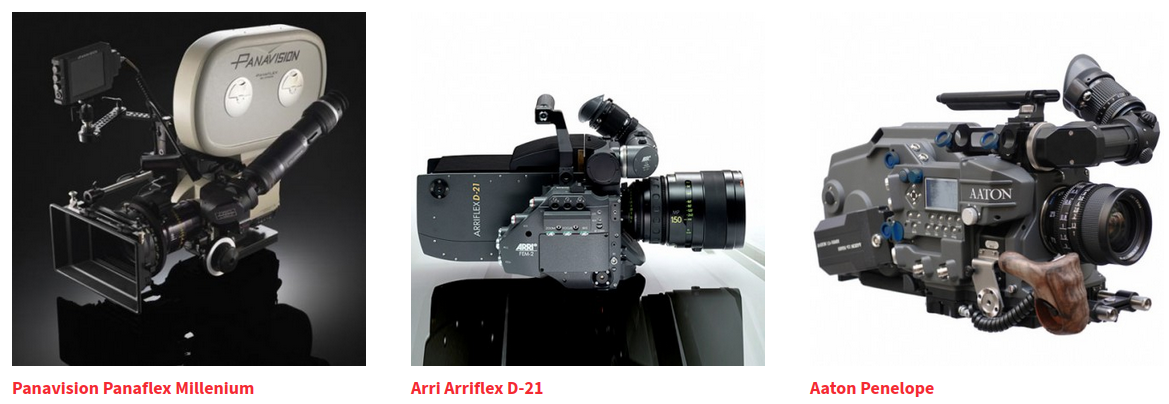
\includegraphics[scale=0.38]{image/professionnel.png}
			\decoRule
			\caption[Caméras professionnel]{image de caméra  professionnel.}
			\label{fig:Caméras professionnel}
		\end{figure}	
		
	\item \textbf{Les Caméras de type "Super Concentré"} « Super Concentré » est un terme inventer dans l'article\cite{noauthor_les_2015} pour catégoriser cette dernière tendance d’appareils. Ce qui les qualifie c’est avant tout de très grands capteurs supérieurs à la majorité des caméras prosommateurs qui leur confère une qualité d’image cinématographique comparable aux caméras professionnelles. Les objectifs sont interchangeables, et sont capables d’exporter les rushs au format RAW qui permet une grande souplesse d’ajustement en post-prod.
	\\
				\textbf{Exemple :\\}
			\begin{itemize}
				\item Camera Red
				\item Camera Blackmagic
				\item Canon C300
			\end{itemize}
			\vspace{1 cm}
			\begin{figure}[th]
				\centering
				\includegraphics[scale=0.38]{image/super consentré.png}
				\decoRule
				\caption[Caméras de type "Super Concentré" ]{Caméras de type "Super Concentré".}
				\label{fig:Caméras de type "Super Concentré"}
			\end{figure}
			
	\item \textbf{Les Caméras dédiées} sont des caméras qui sont particulièrement dédiées à un besoin spécifique comme les caméras miniatures pour les sports extremes ou l’embarcation dans les véhicules motorisés, les caméras à haute cadence pour le slow motion, les caméras 3D, ou encore les caméras drones.\\
				\textbf{Exemple :\\}
			\begin{itemize}
				\item Go Pro
				\item Quadrirotor DJL Phantom 2 Vision
				\item Hercules HD Twist
				\item Panasonic AG 3DA1
			\end{itemize}
			 
			\begin{figure}[h]
				\centering
				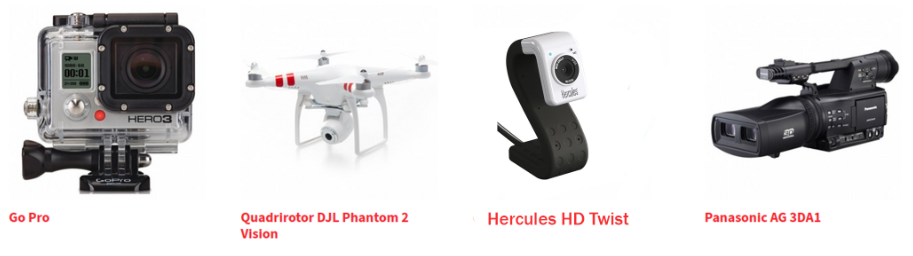
\includegraphics[scale=0.65]{image/caméras dedié.png}
				\decoRule
				\caption[Caméras dedié]{Image de caméras dedié.}
				\label{fig:Caméras dedié}
			\end{figure}
				
\end{itemize}


%----------------------------------------------------------------------------------------
%Notion de calibrage	
%----------------------------------------------------------------------------------------
\newpage
\section{Notion de  Calibrage/étalonnage}

Le calibrage ou étalonnage d'une caméra est tout simplement l’estimation de la relation mathématique existant entre les coordonnées des points 3D de la scène observée et les coordonnées 2D de leur projection dans l'image (points-image),alors calibrer une caméra consiste à estimer sa fonction de transfert.\\

L'estimation de cette relation mathématique est le calcul des différents paramètres de la caméra. C'est une étape nécessaire en vision par ordinateur 3D ou en photogrammétrie afin d'extraire des informations métriques à partir d'images 2D.\\

Il existe deux types de paramètres :\\

  \begin{itemize}
  	\item  Les paramètres internes  du système appelé paramètres intrinsèques composé de:\\
  	
  	\begin{itemize}
  		\item la distance focal
  		\item le centre optique
  		\item les coefficients de distorsion radiale de l'objectif\\
  	\end{itemize}
  	
  	\item Les paramètres externes appelé paramètres extrinsèques :\\
  	
  	\begin{itemize}
  		\item La rotation de la caméra par rapport à un système de coordonnées mondial
  		\item La translation de la caméra par rapport à un système de coordonnées mondial
  	\end{itemize}
  	
  \end{itemize}
 
		\begin{figure}[th]
			\centering
		\includegraphics[scale=0.5]{image/illustration caméras.png}
			\decoRule
			\caption[Illustration d'une caméras]{Schémas d'illustration d'une caméras.}
			\label{fig:Illustration caméras}
		\end{figure}

Pour comprendre l'étalonnage de la caméra , il faut connaitre le modèle de caméra utilisé.

%----------------------------------------------------------------------------------------
%Modèles de caméras	
%----------------------------------------------------------------------------------------
\subsection{Modèles de caméras}
Le modèle utilisé est le modèle sténopé ou « pinhole » en anglais.
ce modèle, aussi connu sous le nom de "camera obscura" ou chambre noire, est un principe optique très ancien qui permet de capturer des images. Il est souvent utilisé pour expliquer les bases de la photographie et les principes fondamentaux de l'optique géométrique. \cite{orteu_calibrage_nodate}
Le modèle sténopé modélise une caméra par une projection perspective. Ce modèle transforme un point 3D de l'espace  en un point-image 2D,c'est une représentation mathématique d'un objet 3D projété dans un espace 2D.\\
 \vspace{-0.3 cm}
 \begin{figure}[h]
 	\centering
 	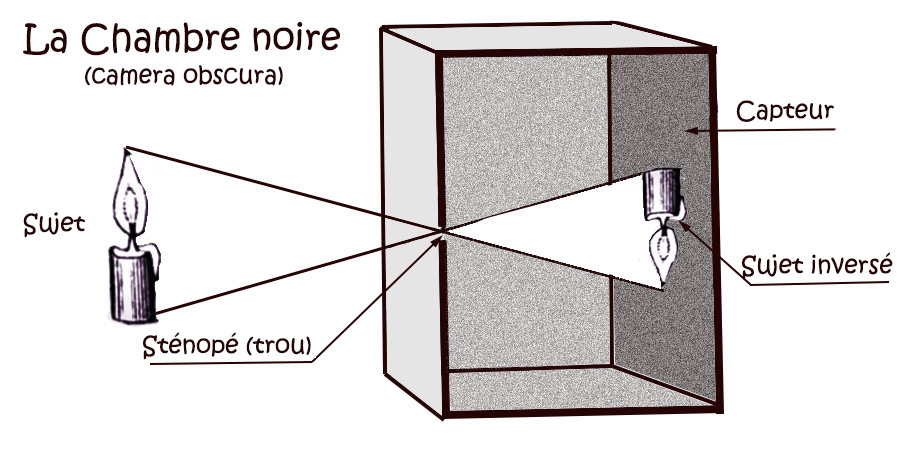
\includegraphics[scale=0.35]{image/chambre-noire.jpg}
 	\decoRule
 	\caption[Modèl sténopé]{Image du modèl sténopé.}
 	\label{fig:Modèl sténopé}
 \end{figure}
  
La figure çi-dessus représente la vision du modèl sténopé \\
par rapport au monde réèl:\\

\begin{itemize}
	\item (x,y,z): repéresente le rèpère orthonormé de centre optique (O)
	\item  Le plan image: qui réprésente le plan de la caméra 
	\item  L'axe optique qui optique qui se trouve sur l'axe Z
	\item  f: qui réprésente la distance focale
	\item  x: qui réprésente la projection d'un point du monde réèl sur le plan image
	\item  X: qui réprésente un point du monde réèl
\end{itemize}
\vspace{-0.3 cm}
\begin{figure}[h]
	\centering
	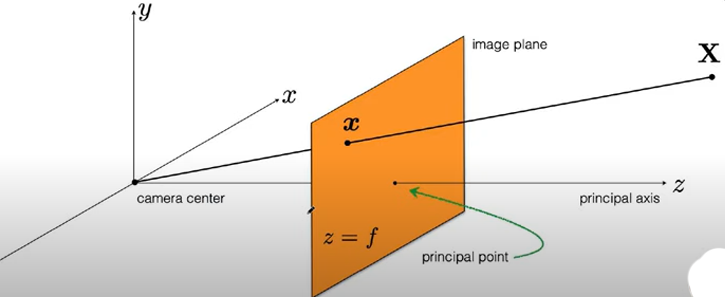
\includegraphics[scale=0.70]{image/ModelStenope.png}
	\decoRule
	\caption[Représentation du modèl sténopé]{Schemas de représentation du modèl sténopé.}
	\label{fig:Représentation du modèl sténopé}
\end{figure}

%----------------------------------------------------------------------------------------
%Les différents techniques de calibrage	
%----------------------------------------------------------------------------------------
\subsection{Les différents techniques de calibrage}

 De nombreux travaux ont été réalisés, à commencer par la communauté de la photogrammétrie et plus récemment en vision par ordinateur.\\
 
 Nous pouvons classer ces techniques grossièrement en deux catégories:\\
 \begin{itemize}
 \item Calibrage photogrammétrique: L'étalonnage est effectué en observant un objet d'étalonnage dont la géométrie dans l'espace 3D est connue avec une très bonne précision. L'étalonnage peut être effectué de manière très efficace. L'objet d'étalonnage est généralement constitué de deux ou trois plans orthogonaux entre eux. Parfois, un plan subissant une translation précisément connue est également utilisé. Ces approches nécessitent un appareil d'étalonnage coûteux et une configuration élaborée \cite{zhengyou_zhang_flexible_1999}.\\
 
 \item Etalonnage en vision par ordinateur: Notre compréhension sur l'étalonnage de la caméra en vision par ordinateur se base sur la littérature de l'article \cite{remondino_digital_2006}. Selon lui les modèles d'étalonnage pour la vision industrielle et par ordinateur utilisent traditionnellement des grilles de référence, la matrice d'étalonnage K étant déterminé à l'aide d'images d'un réseau de points d'objets connu (par exemple un motif en damier). Les méthodes couramment adoptées sont celles de Tsai,Heikkila et Silven  et Zhang \cite{zhengyou_zhang_flexible_1999} Cité dans celui-ci. Ceux­ci sont tous basés sur le modèle de caméra sténopé et incluent des termes pour modéliser la distorsion radiale.\\
 
 \item Auto-calibrage. Les techniques de cette catégorie n’utilisent aucun objet d’étalonnage. En déplaçant simplement une caméra dans une scène statique, la rigidité de la scène fournit en général deux contraintes sur les paramètres internes des caméras à partir d'un déplacement de caméra en utilisant uniquement les informations d'image. Par conséquent, si les images sont prises par la même caméra avec paramètres internes fixes, les correspondances entre trois images suffisent pour récupérer à la fois les paramètres internes et externes qui permettent de reconstruire la structure 3D jusqu'à une similarité \cite{zhengyou_zhang_flexible_1999}.\\
\end{itemize}

%----------------------------------------------------------------------------------------
%Notion de mesure de distance numérique	
%----------------------------------------------------------------------------------------
\newpage
\section{Notion de mesure de distance numérique}


%---------------------------------------------------------------------------------------


















































 

% Chapter 2

\chapter{Implémentation} % Main chapter title

\label{Chapter2} % For referencing the chapter elsewhere, use \ref{Chapter1}

%----------------------------------------------------------------------------------------
%	Structuration du travail
%----------------------------------------------------------------------------------------
%\section{Structuration du travail} 

%\subsection{Feuille de route technologique}

%\subsection{Choix technologique}

\section{Calibrage et correction de la distorsion}
   L'étalonnage de la caméra est généralement 
   perturbé par l'angle, la lumière, l'équipement matériel, 
   etc. Il y a certaines erreurs matérielles et des défauts de conception, qui entraîneront différents degrés et types de distorsion du produit.
   Étant donné que cette recherche consiste à calculer la portée de l'image, 
   l'étalonnage de la caméra et la correction de la distorsion 
   doivent être effectués pour les images prise et pour la vidéo.\\
   La « méthode d'étalonnage de Zhang Zhengyou » est la plus courante et beaucoup utilisé.
      
\subsection{Etude de la méthode de Zhang}
   
   La méthode de calibrage proposé par zhang Zhengyou connue sous le nom méthode de calibrage de caméra basée sur le plan d'échiquier est une technique simple, flexible et réalisable à moindre coût.\\ 
   Cette technique proposée nécessite uniquement que la caméra observe un motif plan affiché dans quelques (au moins deux) orientations
   différentes. Le motif peut être imprimé et fixé sur une surface plane « raisonnable » (par exemple, une couverture de livre rigide).La caméra ou le motif planaire peuvent être déplacés à la main. L'approche proposée se situe entre le calibrage photogrammétrique et l'auto-calibrage car ils utilisent des informations métriques 2D plutôt que 3D ou purement implicites. \\
   
   Dans l'article le travail a été regroupé en quatre sections qui sont:\\
    
   \begin{itemize}
   	\item \textbf{La section 1 (Les contraintes de bases liées à l'observation d'un seul plan):} Comporte la notation de la matrice du caméras et les deux contraintes lié aux paramètres intrinsèques.\\
   	
   	\item \textbf{La section 2 (La procédure de calibrage):}  aborde d'abord la solution fermé qui permet de résoudre les contraintes liées aux paramètres intrinsèques , ensuite la technique d'optimisation non linéaire basée sur le critère du maximum de vraisemblance pour affiner les paramètres avec l'algorithme de Levenberg ­Marquardt et enfin la prise en compte de la distorsion radial de la lentille pour corriger la distorsion.\\
   	
   	\item \textbf{La section 4} étudie les configurations dans lesquelles la technique d'étalonnage proposée échoue\\
   	
   	\item \textbf{La section 5} fournie les résultats expérimentaux.
   \end{itemize}
   
   
   
   
   
%\section{Première partie: Mesure avec le bois}
%\section{Deuxième partie: Intervention d'humain }







 
%\include{Chapters/Chapter3}
%\include{Chapters/Chapter4} 
%\include{Chapters/Chapter5} 

%----------------------------------------------------------------------------------------
%	THESIS CONTENT - APPENDICES
%----------------------------------------------------------------------------------------

%\appendix % Cue to tell LaTeX that the following "chapters" are Appendices

% Include the appendices of the thesis as separate files from the Appendices folder
% Uncomment the lines as you write the Appendices

%% Appendix A

\chapter{Frequently Asked Questions} % Main appendix title

\label{AppendixA} % For referencing this appendix elsewhere, use \ref{AppendixA}

\section{How do I change the colors of links?}

The color of links can be changed to your liking using:

{\small\verb!\hypersetup{urlcolor=red}!}, or

{\small\verb!\hypersetup{citecolor=green}!}, or

{\small\verb!\hypersetup{allcolor=blue}!}.

\noindent If you want to completely hide the links, you can use:

{\small\verb!\hypersetup{allcolors=.}!}, or even better: 

{\small\verb!\hypersetup{hidelinks}!}.

\noindent If you want to have obvious links in the PDF but not the printed text, use:

{\small\verb!\hypersetup{colorlinks=false}!}.

%\include{Appendices/AppendixB}
%\include{Appendices/AppendixC}

%----------------------------------------------------------------------------------------
%	BIBLIOGRAPHY
%----------------------------------------------------------------------------------------

\printbibliography[heading=bibintoc]

%----------------------------------------------------------------------------------------

\end{document}  
